%!TEX root=../oi-magistr-si.tex
\section[AOS - WS]{Webové služby. K čemu slouží? Popis a vyhledávání služeb. Technologie pro implementaci a nasazení služeb a klientů. Protokoly, kódování obsahu. Top-down a bottom-up design}

\subsection{Webové služby}
W3C definice - SW systém designovaný k vzájemné \textit{machine-to-machine} spolupráci přes internet, který má API přístupné přes \textbf{HTTP}, rozhraní je popsáno v strojové čitelném formátu (\textbf{WSDL}) a interakce s WS je pomocí \textbf{SOAP}  zpráv (HTTP + XML).

\paragraph{RPC Web Service} RPC webové služby představují volání vzdálené funkce. Metoda je popsána jako operace ve WSDL. Parametry metody i odpověď jsou posílány jako XML zabalené v SOAP. Vetšinou je implementováno jako mapování služby přímo na jazykově specifické volání funkce. Není tedy loosely coupled.

\paragraph{SOA Web Service} Webové služby se také používají k implementaci SOA, kde je základní jednotkou komunikace zpráva, nikoli operace. Tato skutečnost je často označována jako „message-oriented“ služba.
Na rozdíl od RPC webových služeb jsou SOA webové služby loose coupled, jelikož jsou zaměřeny na kontrakt poskytnutý WSDL, ne na implementační detaily.

\paragraph{RESTfull Web services} RESTfull webové služby jsou speciální podmnožinou webových služeb, které mají sadu předem definovaných operací. Tyto předem definované operace jsou přímo operace převzaté z protokolu HTTP, jedná se tedy o operace GET, POST, HEAD, atd. Každá z operací má vymezené svoje postavení vůči zdroji, který je identifikován pomocí URL. Následující tabulka shrnuje použití jednotlivých HTTP funkcí z pohledu REST služeb.

Využití metod ve správném významu je zcela klíčové pro čisté REST služby. Existuje mnoho reálných implementací webových služeb, kde je právě tento princip porušen.


\subsection{Vyhledávání služeb - UDDI registr}
UDDI (The Universal Description, Discovery and Integration Service) poskytuje mechanismus, přes který mohou klienti dynamicky hledat požadované webové služby. Tímto způsobem by aplikace měly být schopny se kontaktovat na služby poskytované externími partnery. Registr UDDI má dva druhy klientů: ty, kteří chtějí nějakou službu poskytovat a ty, kteří chtějí službu využívat.

\begin{itemize}[itemsep=0px]
\item platformně nezávislý XML-based registr služeb
\item mechanismus pro hledání WS
\item registry:
\begin{itemize}[itemsep=0px]
\item white pages - adresy, kontakty, identifikátory
\item yellow pages - kategorizace servis založena na standartních taxonomiích
\item green pages - technický popis servis (jak k ní přistoupit atd.)
\end{itemize}
\end{itemize}

\begin{figure}[h!]
\centering
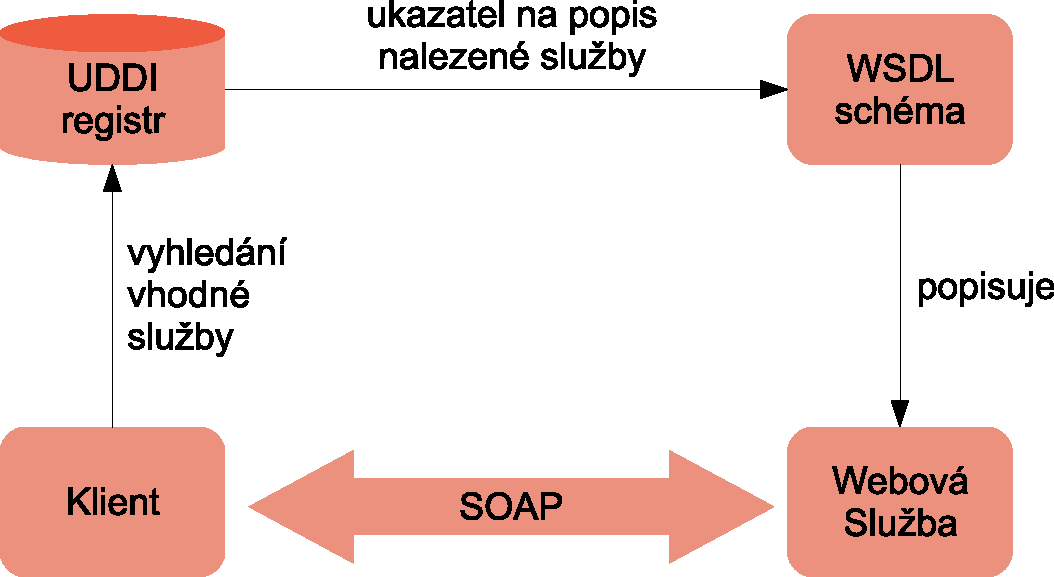
\includegraphics[width=100mm]{10/images/uddi}
\end{figure}

\subsection{Technologie a protokoly}
\subsubsection*{RPC (Remote Procedure Call)}
\begin{itemize}[itemsep=0px]
\item technologie dovolující programu vykonat proceduru (zavolat službu), která může být uložena na jiném místě než je umístěn sám volající program
\item klient/server model
\item synchronní volání klienta - je blokován dokud server neodpoví
\item může nastat chyba v případě chyby sítě
\end{itemize}

\paragraph{Postup} Nejprve proběhne jednoduché zabalení parametrů a identifikátorů procedury do formy vhodné pro přenos mezi počítači (tzv. \textit{marshalling} (serializace)). Poté se balíček odešle. Balíček se na vzdáleném místě rozbalí, zjistí se o jakou proceduru jde (\textit{unmarshalling}). Následuje samotné zavolání a provedení procedury. Výsledek procedury se opět zabalí a odešle zpět. První počítač výsledek opětovně rozbalí. A přijatá hodnota se předá proceduře.

\subsubsection*{CORBA (Common Object Request Broker Architecture)}
\begin{itemize}[itemsep=0px]
\item standard, který umožňuje komunikaci mezi různými platformami a jazyky
\item \hl{jazykově, technologicky a platformě nezávislý}
\item specifikace zahrnuje: silné typování, výjimky, síťový protokol
\item CORBA IDL (Interface Definition Language)
\item transakce, security, marshalling
\end{itemize}

\hl{Je to objektová sběrnice, která objektům umožňuje transparentně vysílat požadavky (requests) směrem k jiným objektům (ať již lokálním nebo vzdáleným) a následně od těchto objektů přijímat odpovědi (replies).} Toto prostředí je nezávislé jak na programovacím jazyce, tak na operačním systému či hardwarové  platformě.

Pro komunikaci mezi CORBA objekty jsou důležité specifikace jejich rozhraní v  jazyce IDL (Interface Definition Language). Ty slouží jako jakási forma kontraktu mezi CORBA objekty a jejich potenciálními klienty jinak řečeno, \hl{klient volá pouze metody nad rozhraním definovaným v IDL, a nestará se o to, jakým způsobem je daný objekt implementován.} IDL specifikace rozhraní jsou následně, s pomocí IDL kompilátoru, mapovány do konkrétních programovacích jazyků, ve kterých jsou již pak dané CORBA objekty implementovány. Použitím tohoto mechanismu dochází k oddělení implementace CORBA objektů od jejich rozhraní, čímž se dosahuje již jednou zmíněné nezávislosti CORBA prostředí na programovacím jazyce.

\paragraph{Volání metod CORBA objektů}
\hl{Vzdálený CORBA objekt} je v klientském adresovém prostoru \hl{zastupován jiným objektem, tzv. \textit{proxy}}. Proxy má obvykle stejné rozhraní jako cílový objekt, a jeho metodami jsou tzv. \hl{\textit{stuby}} (stubs). Stubem se označuje kód, který vezme všechny parametry volání, vloží je spolu s identifikací dané operace do zprávy (marshalling) a tuto zprávu předá jádru ORBu k doručení směrem k cílovému objektu. Na straně serveru předá ORB došlou zprávu skeletonu. Úkolem skeletonu je vyjmout z ní identifikaci požadované operace spolu s jejími parametry, a tuto 
operaci zavolat nad implementací CORBA objektu. Formát zpráv předávaných mezi klientem a serverem je specifikován protokolem  IIOP (Internet Inter-ORB Protocol), který zajišťuje interoperabilitu mezi ORBy různých výrobců.
Z popsaného mechanismu je patrno, že lokální volání metody nad proxy má tedy za následek pro klienta transparentní vyvolání odpovídající metody nad vzdáleným objektem (tento mechanismus již známe z RPC). Poznamenejme pouze, že kód klientského proxy i serverovského skeletonu je automaticky generován IDL kompilátorem na základě popisu rozhraní cílového CORBA objektu \cite{corba}.

\begin{figure}[h!]
\centering
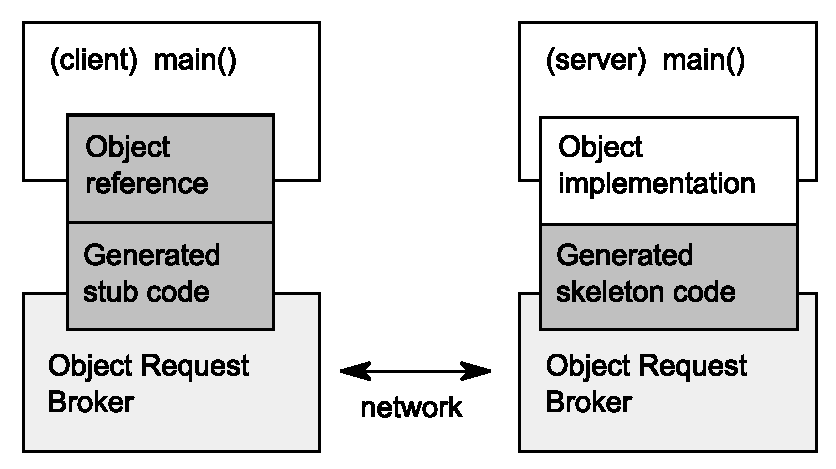
\includegraphics[width=80mm]{10/images/corba}
\caption{CORBA}
\end{figure}

\subsubsection*{DCOM (Distributed Component Object Model)}
\begin{itemize}[itemsep=0px]
\item \hl{microsoftí CORBA} (konkurent)
\item garbage collecting - uvolnění referencí držených klientem (např. při ztrátě spojení)
\end{itemize}
\subsubsection*{WSDL (Web Services Description Language)}
\begin{itemize}[itemsep=0px]
\item \hl{XML-based jazyk, který poskytuje popis (rozhraní) služby}
\item služby jsou definovány jako množina síťových endpointů (portů s adresami a bindováním)
\item popisuje veřejný interface služby
\end{itemize}
\subsubsection*{REST (Representational State Transfer)}
\begin{itemize}[itemsep=0px]
\item architektonický styl nebo množina principů pro tvorbu WS
\item klienti/servery
\item klient se dotáže - server zpracuje požadavek a vrátí odezvu
\item původně popsán pro HTTP (ale není na něj omezen)
\item vlastnosti:
\begin{itemize}[itemsep=0px]
\item stateless
\item cacheable
\item layered system
\item code on demand (opt)
\item uniform interface
\end{itemize}
\end{itemize}
\subsubsection*{SOAP (Simple Object Access Protokol)}
Jelikož veškerá komunikace mezi službami je založená na posílání zpráv, musely být zavedeny takové standardy, aby služby mezi sebou komunikovaly jednotným způsobem. Takovýmto standardem se stal SOAP. SOAP je protokol umožňující spotřebiteli služeb komunikovat s jejich poskytovatelem. Tento protokol je nezávislý na typu sítě, podporuje zprávy ve formátu XML a v současné době je ve specifikaci 1.2 od organizace W3C.

\begin{itemize}[itemsep=0px]
\item specifikace pro výměnu strukturovaných informací pomocí webových služeb
\item SOAP je nezávislý na transportních protokolech. HTTP je jen jedním z podporovaných.
\item postaveno na WSDL a UDDI
\item navrženo jako object-access protokol
\end{itemize}

\begin{wrapfigure}{r}{0.35\textwidth}
  \begin{center}
    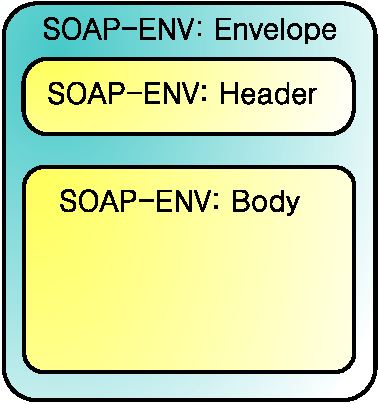
\includegraphics[width=0.28\textwidth]{10/images/soap-message}
  \end{center}
  \vspace{-10px}
  \caption{SOAP zpráva}
\end{wrapfigure}

\paragraph{Struktura zprávy v SOAP}
Každá zpráva dodržující podmínky kladené SOAP je v podstatě balíček (obálka, angl. envelope). Tento balíček obsahuje hlavičku (angl. head) a tělo (angl. body). Hlavička se skládá z několika bloků, které obsahují metainformace. Hlavička je nepovinná (tzn. může být vynechána). Metainformace v sobě ukrývají část komunikační logiky a obecně umožňují zavádět nová rozšíření. Typicky hlavička obsahuje nutné informace pro všechny služby, které mohou zprávu obdržet. Cílová služba potom na základě těchto informací rozhodne o způsobu zpracování zprávy. Tělo obsahuje samotná data (ve formátu XML). Tělo může také obsahovat sekci pro
chyby (angl. faults), která obsahuje logiku pro zpracování výjimek. Většinou jsou v této části uloženy jednoduché zprávy, které slouží k odeslání informací o chybě při výskytu výjimky. SOAP zahrnuje také prostředky pro posílání dat, která jsou těžko popsatelná pomocí XML (binární data, např. obrázky). Takováto data se posílají jako přílohy (angl. attachments).

\subsection{Kódování obsahu}
\hl{Posílaný obsah} je potřeba nějakým způsobem reprezentovat. Požadavky jsou aby \hl{\textbf{reprezentace}} (zakódování) byla lidsky \hl{\textbf{čitelná}, \textbf{neukecaná}} (binary efficient - chceme posílat co nejmenší obsah), platformně \textbf{nezávislá} a \textbf{standardizovaná}.

\begin{itemize}[itemsep=0px]
\item XML - příliš ukecané
\item \hl{JSON - používané}
\item YAML
\item buffers by Google
\end{itemize}

\subsection{Bottom-up design}
Nejdříve je naimplementována služba v konkrétním jazyce, následně je vygenerováno WSDL. Považováno za jednodušší návrh. Riziko vzniku závislosti na programovacím jazyku či platformě.

\subsection{Top-down design}
Nejdřive je napsán WSDL dokument (koresponduje s SOA modelem), následně je z něj vygenerován kód. Považováno za obtížnější. výsledkem je ale čistší design.
